% Packages %%%%%%%%%%%%%%%%%%%%%%%%%%%%%%%%%%%%%%%%%%%%%%%%%%%
\documentclass[conference]{IEEEtran}
\IEEEoverridecommandlockouts 
\usepackage{cite}
\usepackage{xfrac}
\usepackage[cmex10]{amsmath}
\usepackage{amssymb}
%\usepackage{algorithmic}
\usepackage{array}
\usepackage{mdwmath}
\usepackage{mdwtab}
\usepackage{eqparbox}
\usepackage{graphicx}
\usepackage[]{subfigure}
\usepackage{url}
\usepackage[algoruled,vlined,linesnumbered]{algorithm2e}
\usepackage{verbatim}
\usepackage{color}
\usepackage{hyperref}
\usepackage{mathtools}


\makeindex 
\makeatletter

%%%%%%%%%%%%%%%%%%%%%%%%%%%%%%%%%%%%%%%%%%%%%%%%%%%%%%%%%%%%%%%%
% Magic stuff to shrink stuff
\makeatletter
\renewcommand\section{\@startsection{section}{1}{\z@}
                                  {-3.0ex plus -1.5ex minus -0.5ex}
                                  {0.7ex plus 1ex minus 0ex}
                                  {\bfseries}}
\renewcommand\subsection{\@startsection{subsection}{1}{\z@}
                                  {-2.0ex plus -1.5ex minus -0.5ex}
                                  {0.7ex plus 1ex minus 0ex}
                                  {\itshape\bfseries}}
\makeatother


%\newcommand{\shrinka}{\def\baselinestretch{0.99}\large\normalsize}

\long\def\IGNORE#1{}


%%%%%%%%%%%%%%%%%%%%%%%%%%%%%%%%%%%%%%%%%%%%%%%%%%%%%%%%%%%%
% Paper Info
\author{ Valerie Bazie $\quad\quad$ Carol Young $\quad\quad$ Ana Huam\'an Quispe%
	\thanks{The authors are with the Georgia Institute of
	Technology, Atlanta, GA 30332, USA. Email:
	{\tt\small vbazie3@gatech.edu},{\tt\small cyoung77@gatech.edu},
	{\tt\small ahuaman3@gatech.edu} }}
\title{ {ECE8843} {P}roject {R}eport 1 : {M}apping an Indoor Environment with a {M}obile {A}utonomous {P}latform }  
%%%%%%%%%%%%%%%%%%%%%%%%%%%%%%%%%%%%%%%%%%%%%%%%%%%%%%%%%%%%
% Document
\begin{document}
\maketitle
%%%%%%%%%%%%%%%%%%%%%%%%%%%%%%%%%%%%%%%%%%%%%%%%%%%
%% Problem Statement
\section{Problem Statement}
Our objective to design a swarm of autonomous mobile
systems that will be able to perform the following:

\begin{enumerate}
\item{ Identify the object to find (which will be presented by a human) }
\item{Two of the robots, seekers, search for an object in an indoor environment, which may
not be known beforehand but the object is within the robot reach }
\item{ The seekers move towards the object and signal a third robot that they have reached it(using
a sound signal such as a beep or some visual cue) }
\item{The third robot, confirmer, navigates towards the object}
\item{The confirmer has a better sensor suite than the seeker and tells if it is indeed the specific object}
\item{(Optionally) The robots should be able to come back to their 
initial position}
\end{enumerate}

%%%%%%%%%%%%%%%%%%%%%%%%%%%%%%%%%%%%%%%%%%%%%%%%%%%
%% Section Simulation Environment
\section{Simulation Environment}
\label{sec:Environment}


%%%%%%%%%%%%%%%%%%%%%%%%%%%%%%%%%%%%%%%%%%%%%%%%%%%
%% Section Algorithms
\section{Algorithms}
\label{sec:Algorithms}

%*********************************
\subsection{Basic Path Search}
\label{sec:BasicSearch}
Our robots interact in a 3D environment. However, it
is common practice to simplify the problem by considering
movements in a 2D space. Details of our chosen approach
are shown below:

\begin{itemize}
\item{\textit{Approach considered:} $A^{*}$}
\item{\textit{Environment representation:} 8-neighbor grid}
\item{\textit{Discretization level:} Grids of $10\text{ cm} \times 10\text{ cm}$}
\item{\textit{Space considered:} $8\text{ m} \times 8\text{ m}$}
\item{\textit{Additional considerations:} Partially known environment
at starting time}
\end{itemize}

%*********************************
\subsection{Object Identification}
\label{sec:ObjectIdentification}
Our perception from the world comes from two sources:
\begin{itemize}
\item{\textit{Visual data:} Kinect}
\item{\textit{Sonar data}: Relative localization between robots}
\end{itemize}

In this section, we are concerned with visual
object identification. For sake of simplicity
we follow the following assumptions:

\begin{itemize} 
\item{Robots have a distinctive color feature
that allows our visual system to recognize them}
\item{No other object on the environment possess
the feature mentioned above}
\end{itemize}

The easiest approach to identify an object with the
conditions above is a straightforward blob-detection
method. Rather than implementing this from scratch,
we intend to use the OpenCV free implementation of this method\footnote{http://opencv.willowgarage.com/wiki/cvBlobsLib}.
\medskip

A potential problem we might have with using blob
detection is detection robustness under different
illumination conditions. Given this, we further restrict
our test scenario to be an indoor environment with fixed
lighting.

%*********************************
\subsection{Seeker Dynamic Signal}
\label{sec:SeekerDynamicSignal}
The seeker robots are in charge of finding the desired object,
move towards it and inform to the remaining robot
of the likely location of the target. A block diagram of this 
process is shown in Fig.\ref{fig:Seeker}:

%------------------------------------------------------------
% Image: Seeker
\begin{figure}[h]
	\centering
	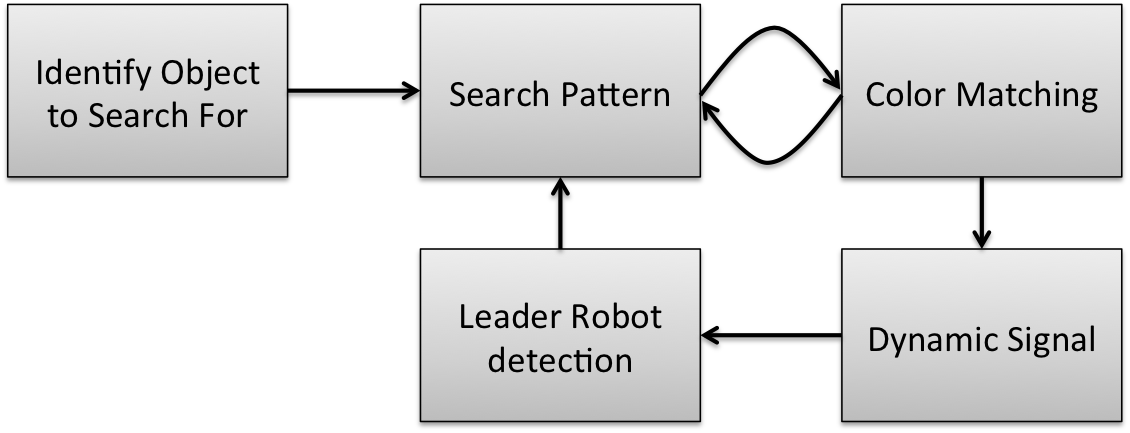
\includegraphics[height=90pt]{images/Seeker_Block.png} 
	\label{fig:Seeker}
    \caption{Seeker process}
\end{figure}

And the pseudocode is shown below:
\medskip

\begin{itemize}
\item{Identify correctly colored object}
\item{Maneuver object to center of field of view}
\item{If object was to right of center increase left wheel speed proportionally
	\begin{itemize}
		\item{Opposite if object was to the left of center}
	\end{itemize} }
\item{Rotate $180^{\circ}$ using odometry information} 
\item{Accelerate forward at $2 \sfrac{m}{s^{2}}$ for $0.5$ seconds}
\item{Accelerate at $-2 \sfrac{m}{s^{2}}$ for 1 second}
\item{Accelerate at $2 \sfrac{m}{s^{2}}$ for 1 second}
\item{Repeat Acceleration cycle}
\item{Slow to $\pm1 \sfrac{m}{s^{2}}$ acceleration when an object moves to within $1$ meter in front of it}
\item{Stop at starting point when the object moves to within $0.5$ meters in front of it}
\item{Continue Search pattern when object moves to within $0.25$ meters for 3 seconds}
\end{itemize}

%*********************************
\subsection{Leader Identify Dynamic Signal}
\label{sec:LeaderIdentifyDynamicSignal}
The leader robot is in charge of correctly identifying 
the desired object. Fig.\ref{fig:Leader} shows a block
diagram of this process, which is explained in this and the
following subsections:

%------------------------------------------------------------
% Image: Leader
\begin{figure}[h]
	\centering
	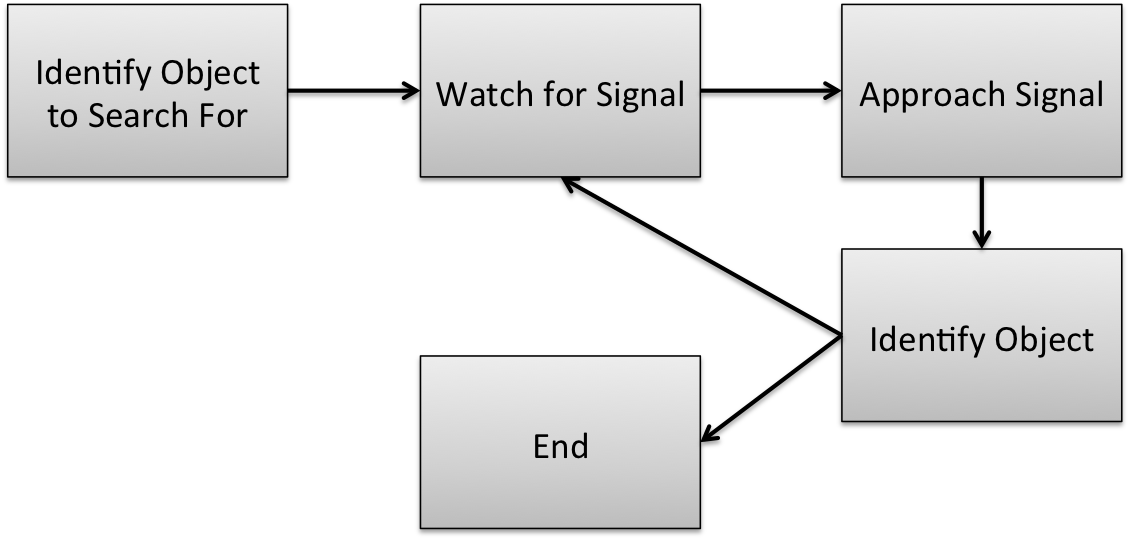
\includegraphics[height=90pt]{images/Leader_Block.png} 
	\label{fig:Leader}
    \caption{Leader block diagram}
\end{figure}

For signal identification, the pseudocode is shown below:

\begin{itemize}
\item{At initial time step note location of all 3D objects in field of view $p_{t}$}
\item{At $(t+1)$ note location of 3D objects $p_{t+1}$}
\item{Compare $p_{t}$ and $p_{t+1}$ any objects within 10cm are the same object and standing still and remaining detected objects are matched with closest in each other sets set $p_{t}$  and $p_{t+1}$ that match each other are the same object that has moved.  And note the change in position (Velocity)}
\item{At $(t+2)$ repeat $p_{t+1}$ steps and also note the change in the change in velocity (acceleration)}
\item{If acceleration is $>$ $1 \sfrac{m}{s^{2}}$ start moving towards object
	\begin{itemize}
		\item{Else if number of moving objects is less than $2$, change adjust field of view by rotating and then repeat}
		\item{Else repeat} 
	\end{itemize} }
\end{itemize}

%*********************************
\subsection{Leader Move Towards Dynamic Signal}
\label{sec:LeaderMoveTowardsDynamicSignal}

Once signaling robot is identified
\begin{itemize}
\item{Record positions of robot for 2 seconds}
\item{Note location of largest distance and smallest distance}
\item{Move towards position of smallest distance}
\item{When distance between leader and seeker is less than .5 m once move towards current seeker location}
\item{When distance between leader and seeker is less than .25 m stop.}
\item{Start slow turn using camera to find colored object}
\item{Center color in center of the frame}
\item{Use Kinect to identify object}
\item{If correct stop}
\item{If incorrect continue Leader Identify Dynamic Signal}
\end{itemize}

%*********************************
\subsection{3D 0bject Localization}
\label{sec:Localization}
In section \ref{sec:ObjectIdentification} we
briefly explained our approach to object identification in
the image. The next step is the ability to place the
object in a 3D world location that give the robots the needed
information to do a path search to reach that location.

For this step, we use the RGB-D information provided by Kinect.
Once the pixels belonging to the objects are identified, we can
retrieve the distance from the object to our robot (up to 8 meters).
Since this signal may be noisy we will constantly update the distance
information. 

As an additional step, we may partially reconstruct the 3D environment,
since we know beforehand the camera calibration parameters, so it is possible
to perform the reconstruction of the environment (using as a reference the 
starting location of the robot).

\end{document}